\subsection{Основные определения.}

Начнем с определений. 

\deff{def:} $V$ - линейное пространство над полем $\mathbb{R}$.

$(\cdot, \cdot ): V\times V \xrightarrow{} \R$ называется \deff{скалярное произведение}, если она удовлетворяет 4-ем аксиомам.

$\forall x,y \in V$, $\forall \lambda \in \R$:

\begin{enumerate}
    \item $(x,y) = (y,x)$ --- симметричность
    \item $(x_1 +x_2,y) = (x_1,y)+(x_2,y)$
    \item $(\lambda x, y) = \lambda (x,y)$
    \item $\forall x \neq 0: (x,x)>0$
\end{enumerate}

\deff{def:} $(V, (\cdot, \cdot))$ $\dim V =n<\infty$ называется \deff{евклидовым пространством} или вещественным линейным пространством со скалярным произведением.

\textbf{Замечание:} Если $V$ бесконечномерно, то это называется \deff{гильбертовым пространством}

\deff{def:} $V$ - линейное пространство над полем $\C$.

$(\cdot, \cdot): V\times V \xrightarrow{} \C$ функция называется \deff{псевдоскалярным} пространством.

\begin{enumerate}
    \item $(x,y) = \overline{(y,x)}$ --- симметричность
    \item $(x_1 +x_2,y) = (x_1,y)+(x_2,y)$
    \item $(\lambda x, y) = \lambda (x,y)$
    \item $\forall x \neq 0: (x,x)>0$
\end{enumerate}

Такая функция называется \deff{полуторалинейной}.

\deff{def:} $\dim V = n < \infty$, $(V, (\cdot, \cdot))$ называется \deff{унитарным} пространством или эрмитовый или псевдоевклидовой или комплексным линейным пространством с псевдоскаляром.

\textbf{Замечание:} Если вы не напишите слово вещественные или комплексные в работе или на экзамене, то вам инста бан.

\deff{def:} Введем норму: $\forall x \in V: ||x|| =\sqrt{(x,x)}$ --- \deff{евклидова норма}.

Давайте проверим выполняемость свойств нормы.

\begin{enumerate} %todo
    \item $\forall x \neq 0 \Rightarrow ||x|| \neq 0$ (невырожденность) --- выполнена.
    \item  $\forall \lambda \in K \Rightarrow ||\lambda x|| = \sqrt{(\lambda x, \lambda x)} = |\lambda|\cdot||x||$ (однородность) --- выполнено.
    \item  $\forall x, y\in V$ неравенство треугольника. 
    $$||x+y||\leq ||x|| + ||y||$$
    Мы будем пользоваться в доказательстве неравенством КБШ. Его доказательство вы можете найти в конспекте первого семестра по матанализу. 
    $$||x+y||^2 = (x+y,x+y) = ||x||^2 + (x,y) + (y,x) + ||y||^2 \leq ||x||^2 + 2 Re(x,y) + ||y||^2 \leq$$
    $$\leq ||x||^2 + 2||x||\cdot||y|| + ||y||^2 \leq  (||x|| + ||y||)^2$$
    $$\Rightarrow ||x+y|| \leq ||x|| + ||y||$$
\end{enumerate} 

\deff{def:}  $\forall x \in V:$ $||x||$ - \deff{длина вектора}. $\varphi$ называем углом между $x$ и $y$, таким, что $\cos \varphi = \cfrac{(x,y)}{||x||||y||}$

\textbf{Пример:}

\begin{enumerate}
    \item Возьмем $\mathbb{R}^n$. $\forall x,y \in \C^n$. $(x,y) = \sum\limits_{i=1}^n x_i \overline{y_i}$. Заметим что выполнены все 4 аксиомы скалярного произведения
    $$||x|| = (\sum\limits_{i=1}^n |x_i|^2)^{1/2} = \sqrt{(x,x)} = \sqrt{\sum\limits_{i=1}^n x_i \overline{x_i}}$$
    Неравенство КБШ в данном случае будет вот таким:
    $$\sum\limits_{i=1}^n |x_iy_i| \leq \left(\sum\limits_{i=1}^n |x_i|^2\right)^{\cfrac{1}{2}} \cdot \left ( \sum\limits_{i=1}^{n} |y_i|^2\right)^{\cfrac{1}{2}}$$
    А неравенство треугольника у нас будет вот таким:
    $$\left(\sum\limits_{i=1}^n|x_i+y_i|^2\right)^{\cfrac{1}{2}}\leq \left(\sum\limits_{i=1}^n|x_i|^2\right) ^{\cfrac{1}{2}} + \left(\sum\limits_{i=1}^n |y_i|^2\right)^{\cfrac{1}{2}}$$
    По-другому неравентво треугольника в данном случае будет называться неравенством Минковского.
    \item Так же мы будем пользоваться вот таким примером. Пусть у нас выбран промежуток $[a,b]$ и $\integral{a}{b}|f|^2dt < \infty$. Тогда введем скалярное произведение: 
    $$(f,g) = \integral{a}{b} f \overline{g}dt$$
\end{enumerate}

\pagebreak
\subsection{Процесс ортогонализация Грама-Шмидта. Орто-нормированный базис. Ортогональное дополнение.}

\deff{def:} Cистема ненулевых векторов $v_1,\ldots, v_m$ называется \deff{ортогональным}, если $\forall (i,j), i\neq j: (v_i,v_j) =0$.  



\deff{def:} Система ненулевых векторов называется \deff{ортонормированной}, если $v_1,\ldots, v_m: \forall (i,j): (v_i,v_j) = \delta_{ij}$. $||v_i||= 1$

\deff{Утверждение:} $v_1,\ldots, v_m$ ортогональная $\Rightarrow$ $v_1,\ldots , v_m$ \uline{линейно независимы}.

\textbf{Доказательство:}

$v_1,\ldots, v_m$ ортогональны. Хотим показать тривиальность разложения нуля(в принципе ничего нового).
$$\sum\limits_{i=1}^n \alpha_i v_i =\zero$$
Давайте применим операцию скалярного произведения с $v_j$ к обеим частям. Таким образом получим:
$$0 = \sum\limits_{i=1}^n \alpha_i (v_i,v_j)= \alpha_j (v_j,v_j) \Rightarrow \alpha_j =0$$ 
Таким образом получаю, что каждая $\alpha_j = 0$, то есть вектора линейно независимы.

\hfill Q.E.D.


\thmm{Теорема (процесс ортогонализации Грама-Шмидта)}

$\forall a_1,\ldots,a_n \rightarrow \exists b_1,\ldots,b_k \in V$. Причем $b_i$ попарно-ортогонально и $\span (a_1,\ldots, a_n) = \span(b_1,\ldots,b_k)$. При этом $k = \rg (a_1,\ldots,a_m)$

\textbf{Доказательство:}

Пусть $a_1,\ldots,a_m$ линейно независимы, то есть $m=k$

Будем доказывать по индукции.

\textbf{База:}

Рассмотрим $k=2$, пусть $b_1 = a_1$. Мы хотим, чтобы $b_2$ и $b_1$ были ортогональны, то есть $(b_1,b_2) = 0$. Пусть $b_2 = a_2 - c_1 b_1$. Тогда, нам надо, чтобы было выполнено:
$$0 = (b_2,b_1) = (a_1,b_1)-c_1(b_1,b_1) \Leftrightarrow c_1 = \cfrac{(a_2,b_1)}{(b_1,b_1)}$$
Заметим, что сейчас мы нашли такое $b_2$, что оно ортогонально и тк мы сделали линейное преобразование, то $\span (b_1,b_2) = \span (a_1,a_2)$

\textbf{Индукционный переход:}

Пусть верно для $m$. Докажем для $m+1$.

Возьму первые $m$. Для них по предположению индукцию построю ортогональные.

Возьму $b_{m+1}=a_{m+1} - \sum\limits_{j=1}^m c_j b_j$

Хотим, понять существуют ли такие $c$. Давайте переберем $r = 1\ldots m $ и возьмем скалярное произведение с $b_r$. Тогда:
$$0 = (b_{m+1}, b_r) = (a_{m+1},b_r)-\sum\limits_{j=1}^m c_j(b_j,b_r) = (a_{m+1},b_r)-c_r(b_r,b_r)$$
$c_r = \cfrac{(a_{m+1}, b_r)}{||b_r||^2}$

Заметим, что $b_{m+1}\neq 0$, тк иначе $a_{m+1}\in \span(b_1,\ldots b_n)$, откуда линейно-независимый. Откуда получили $m+1$ ортогональный.

\hfill Q.E.D.

\textbf{Следствие 1:} Для любого пространства $V$ евклидова, унитарного всегда существует ортонормированный базис.

\textbf{Следствие 2:} Любую ортогональную систему в $V$ можно дополнить до о.н.б.

\deff{def:} $L \subset V$ $L^{\perp} = \{y \in V | (x,y)=0, \forall x \in L\}$
--- \deff{ортогональное дополнение} $L$.

\textbf{Свойства:}
\begin{enumerate}
    \item $L^{\perp}$ --- линейное подпространство. 
    $$\forall y_1,y_2 \in L^{\perp}, \forall \lambda \in K: (x,\lambda y_1 + \lambda y_2) = \overline{\lambda} (x,y_1) + (x,y_2) = 0$$
    Откуда $\lambda y_1  + y_2 \in L^{\perp}$

    \item $V = L \oplus L^{\perp}$. 

    \textbf{Доказательство:}

    $L$ и $L^\perp$ очевидно дизъюнктны. Хотим понять $L \oplus L^{\perp}$. Пусть $L = \span (a_1,\ldots,a_n)$ - ортогональный базис $L$. Дополним до базиса $V$. $$V = \span(a_1,\ldots,a_k,a_{k+1},\ldots, a_n)$$
    Тогда очевидно, что $L^\perp = \span (a_{k+1}, \ldots,a_n)$, тк $y = \sum\limits_{j=1}^{n-k} c_j a_{k+j}$ и $\forall x\in L: (x,y) = \sum\limits_{j=1}^{n-k}\overline{c_j}(x, a_{k+j}) = \sum\limits_{j=1}^{n-k}\sum\limits_{m=1}^k \overline{c_j}\alpha+m (a_m,a_{k+j})=0$

    Откуда по эквивалентному условию прямой суммы верно.

    \hfill Q.E.D.

    \textbf{Замечание:} $\forall L: \exists L'$ - прямое дополнение и $\exists L^{\perp}$ со свойством, что его элементы $\perp L$. 

    \item $(L_1+L_2)^\perp = L_1^\perp \cap L_2^\perp$ и $(L_1 \cap L_2)^\perp = L_1^{\perp}+ L_2^{\perp}$

    \textbf{Доказательство:}

    $(L_1+L_2)^{\perp} = L_1^{\perp} \cap L_2^{\perp}$.

    Докажем сначала вложенность в левую сторону:

    $\forall  y \in L_1^\perp \, \&\, y\in L_2^\perp \Leftrightarrow y\in L_1^\perp \cap L_2^\perp$. Как мы знаем:
    $$\forall x_1 \in L_1: (x_1,y)=0$$
    $$\forall x_1 \in L_1: (x_2,y)=0$$
    $$\Rightarrow x_1 + x_2 \in L_1 + L_2; (x_1 + x_2, y) = (x_1,y) + (x_2,y)=0$$
    Откуда $y\in (L_1+L_2)^\perp$.

    Докажем вложенность в правую сторону:

    Пусть $y \in (L_1 + L_2)^\perp \Rightarrow \forall x_1 + x_2 \in L_1 + L_2,x \in L_1, x_2 \in L_2$: $(x_1+x_2,y)=0$. Пусть $x_2 = \zero$. Тогда $\forall x_1 \in L_1: (x_1 + y)=0$. Откуда $y \in L_1^\perp$, аналогично $y \in L_2^\perp$. А это то что нам надо

    Теперь докажем второе равенство:
$$(L_1 \cap L_2)^\perp = L_1^{\perp}+ L_2^{\perp}$$
    Применим первое свойство к $L_1^{\perp}$ 
    $$(L_1^\perp + L_2^\perp)^\perp = (L_1^\perp)^\perp \cap (L_2^\perp)^\perp$$
  А еще:
    $$(L_1^\perp + L_2^\perp)^\perp = L_1 \cap L_2$$
    Поэтому приравняем правые части равенств и получим то, что нам надо
    
    
    \hfill Q.E.D.
    \item $V^\perp  = \zero$
\end{enumerate}

\pagebreak
\subsection{Матрица Грама и ее свойства. Ортогональные и унитарные матрицы.}

Дано $(V, (\cdot,\cdot))$ - евклидово или унитарное, $e$ - базис $V$. $e=(e_1,\ldots, e_n)$.

$\forall x,y \in V: (x,y) = (\sum\limits_{i=1}^n x_i e_i, \sum\limits_{j=1}^n y_i e_j) = \sum\limits_{i=1}^n\sum\limits_{j=1}^n x_i \overline{y_i} (e_i, e_j)$

\deff{def:} $\Gamma  = ((e_i,e_j))_{n\times n} = \begin{pmatrix}
    (e_1,e_1) & \ldots & (e_1, e_n)\\
    \vdots & &\vdots\\
    (e_n,e_1) & \ldots & (e_n,e_n)
\end{pmatrix}$ --- \deff{матрицей Грама}(базиса пространства $V$)

Очевидно, что $\overline{\Gamma^T}  = \Gamma$ из свойств скалярного произведения.

\deff{def:} $A = (a_{ij})_{n \times n}, a_{ij} \in K$. $A^* = \overline{A^T}$ называется матрицей, \deff{сопряженной} к $A$.

\textbf{Замечание:} все $def$ пишем для $\mathbb{C}$, для $\R$ надо убрать операцию сопряжения.

\deff{def:} $A^* = A$ называется \deff{самосопряженной}.
\begin{enumerate}
    \item[$\R$] $A^T = A$ --- симметричная.
    \item[$\C$] $\overline{A^T}=A$  --- \deff{эрмитова матрица}.
\end{enumerate}

$(x,y)   = x^T \cdot \Gamma \cdot \overline{y}$

\textbf{Частный случай.} $e$ - ортонормированный базис $\Gamma = E$.

\textbf{Частный случай.} $e$ - ортогональный базис $\Gamma = diag(||e_1||^2,\ldots,||e_n||^2)$

\deff{def:} Пусть есть $a_1,\ldots, a_k\in V$. Назовем $G = (a_1,\ldots,a_k) =((a_i,a_j))_{k\times k}$ \\--- \deff{матрицей Грама системы векторов}.

Очевидно, что $G^* = G$ - самосопряженная.

Очевидно, что $\Gamma = G(e_1,\ldots, e_n)$ - матрица Грама частный случай.

\deff{def:} $g(a_1,\ldots, a_k) = \det G(a_1,\ldots, a_k)$.

\thmm{Теорема (об определителе матрицы Грама)}

$a_1,\ldots, a_k$ по Граму-Шмидту переводится в попарно-ортогональные $b_1,\ldots,b_k$ (но возможно есть нули).

Тогда $g(a_1,\ldots, a_k) = ||b_1||^2\ldots ||b_k||^2 = g(b_1,\ldots,b_k)$

\textbf{Доказательство:}
$$g(a_1,\ldots, a_k) = \begin{vmatrix}
    (a_1,a_1) & (a_1, a_2) & (a_1,a_3) & \ldots & (a_1,a_n)\\
     (a_2,a_1) & (a_2, a_2) & (a_2,a_3) & \ldots & (a_1,a_n)\\
      (a_3,a_1) & (a_3, a_2) & (a_3,a_3) & \ldots & (a_1,a_n)\\
      \vdots & \vdots & \vdots & & \vdots \\
       (a_n,a_1) & (a_n, a_2) & (a_n,a_3) & \ldots & (a_n,a_n)\\
\end{vmatrix}$$
По процессу ортогонализации я заменяю $a_1$ на $b_1$ получу:
$$g(a_1,\ldots, a_k) = \begin{vmatrix}
    (b_1,b_1) & (b_1, a_2) & (b_1,a_3) & \ldots & (b_1,a_n)\\
     (a_2,b_1) & (a_2, a_2) & (a_2,a_3) & \ldots & (a_1,a_n)\\
      (a_3,b_1) & (a_3, a_2) & (a_3,a_3) & \ldots & (a_1,a_n)\\
      \vdots & \vdots & \vdots & & \vdots \\
       (a_n,b_1) & (a_n, a_2) & (a_n,a_3) & \ldots & (a_n,a_n)\\
\end{vmatrix}$$
Выполним второй шаг. $b_2 = a_2 -c_1$, где $c_1 = \cfrac{(a_2,b_1)}{||b_1||^2}$.

Из второй строки вычту 1 строку умноженную на $c_1$ получу:
$$g(a_1,\ldots, a_k) = \begin{vmatrix}
    (b_1,b_1) & (b_1, a_2) & (b_1,a_3) & \ldots & (b_1,a_n)\\
     (b_2,b_1) & (b_2, a_2) & (b_2,a_3) & \ldots & (b_1,a_n)\\
      (a_3,b_1) & (a_3, a_2) & (a_3,a_3) & \ldots & (a_1,a_n)\\
      \vdots & \vdots & \vdots & & \vdots \\
       (a_n,b_1) & (a_n, a_2) & (a_n,a_3) & \ldots & (a_n,a_n)\\
\end{vmatrix}$$
А теперь из второго столбика вычту первый умноженный на $\overline{c_1}$. Аналогично дальше. Откуда получили то, что нам надо.

\hfill Q.E.D.

\textbf{Следствие 1:} $a_1,\ldots a_k$ - линейно-независимо $\Leftrightarrow$ определитель матрицы Грама $>0$.

\textbf{Следствие 2:} $a_1,\ldots a_{k-1}$ линейно независимы, есть $a_k$. Тогда: $||b_k||^2 = \cfrac{g(a_1,\ldots ,a_k)}{g(a_1,\ldots,a_{k-1})}$.

\deff{def:} $A = (a_{ij})_{n\times n} = \begin{pmatrix}
        a_{11} & \ldots & a_{1k} & \ldots & a_{1n}\\
        \vdots & & \vdots & & \vdots\\
        a_{k1} & \ldots & a_{kk} & \ldots & a_{kn}\\
        \vdots & & \vdots & & \vdots\\
        a_{n1} & \ldots & a_{nk} &\ldots & a_{nn}
    \end{pmatrix}$

\deff{Угловым минором k-ого порядка} называется $\Delta_k = \det A_k = \begin{vmatrix}
    a_{11} & \ldots & a_{1k} \\
    \vdots & & \vdots \\
     a_{k1} & \ldots & a_{kk}
\end{vmatrix}$

\textbf{Свойства} $\Gamma$:
\begin{enumerate}
    \item $\Gamma >0$ \deff{положительно-определенная}. $\Leftrightarrow \begin{cases}
        \Gamma = \Gamma^*\\
        \forall x \in K^n, x^T \Gamma \overline{x} >0 
    \end{cases}$

    Верно из свойств скалярного произведения.   

    \item Для матрицы $\Gamma$ все угловые миноры $\Delta_k >0$. Откуда матрица $\Gamma$ --- невырожденная.

    \item $e,e'$ базисы $V$. $\Gamma = G(e_1,\ldots ,e_n), \Gamma' = G(e_1',\ldots,e_n')$. $\Gamma' = T^T\Gamma \overline{T}$

    \textbf{Доказательство:}

    $\forall x,y \in V: (x,y) = x^T \Gamma \overline{y}$.

    Сделаем замену $x^T \Gamma \cdot \overline{y}  = (x')^T T^T \Gamma \overline{T}\cdot \overline{(y')}= (x')^T \Gamma' \overline{y'}$

    Пусть $x' = E_i, y' = E_j$, тогда подставляя мы получаем поэлементное равенство матриц, откуда доказали

    \item $e,e'$ о.н.б. $V \Rightarrow T^T \overline{T} = E$

\end{enumerate}

\deff{def:} $Q_{n\times n}$ невырожденная. $Q$ называется унитарной, ортогональной, если $Q^* = Q^{-1}$

\textbf{Свойства ортогональной/унитарной матрицы}

\begin{enumerate}
    \item строки и столбцы попарно-ортогональны и нормированны. (со стандартный ск. п.)

\textbf{Доказательство:}
    $$Q^* Q = E = Q Q^*$$
    $$(\overline{Q^T} Q ) =E = (Q \overline{Q^T})$$
    А это получается, что $(Q_i,Q_j) = \sigma_{ij}$, аналогично $(Q_i^T,Q_j^T) = \sigma_{ij}$

    \hfill Q.E.D.

    \item $Q$ ортог/унитар $\Rightarrow Q^{-1}$ ортог/унитар.

    \item $Q,R$ ортог/унитар $\Rightarrow QR$ ортог/унитар.
    \item $|\det Q | = 1 :(\R: \det Q = \pm 1 )$
    \item $e,e'$ о.н.б $\Leftrightarrow$ $T_{e\rightarrow e'}$ ортогонально унитарно

    \textbf{Доказательство:}
    
    $e'$ - о.н.б $\Leftarrow$ $e$ - орто нормированный базис и $T_{e\rightarrow e'}$ - ортог/унитар. - 4-ое свойство матрицы Грама.

    \hfill Q.E.D.

    Я не совсем понял, что тут исправляла ЕА, так что скажите.

\end{enumerate}

\pagebreak
\subsection{Теорема Пифагора. Расстояние до линейного подпространства. Задача о перпендикуляре(наилучшем приближении). Объем k-мерного параллелепипеда в n-мерном пространстве}

\thmm{Теорема (Пифагора)}

$\forall y,z \in V: (y,z) = 0 \Rightarrow ||y+z||^2 = ||y||^2 + ||z||^2$

\textbf{Доказательство:}

$$||y+z||^2 = (y+z,y+z) = (y,y) + (y,z) + (z,y) + (z,z)$$

\hfill Q.E.D.

\textbf{Следствие:} $\forall x_1,\ldots ,x_k \in V$ попарно-ортогональными: $||\sum\limits_{j=1}^k x_j||^2 = \sum\limits_{j=1}^k||x_j||^2$


\deff{def:}
\begin{center}
   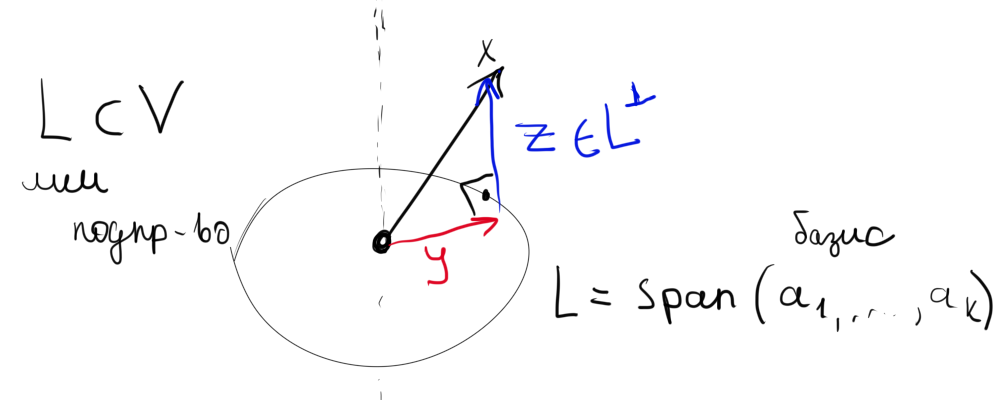
\includegraphics[width = 10 cm]{assets/9_4-orthogonal-projection.png}
\end{center}

$V = L \oplus L^\perp$. $\forall x \in V: x = y + z$ представляется единственным образом, где $y\in L, z\in L^\perp$. В таком случае $y$ называется \deff{ортогональной проекцией} $x$ на линейное подпространство $L$. $z$ - \deff{ортогональная составляющая} $x$ относительно линейного подпространства $L$ или \deff{перпендикуляром}, опущенным из $x$ на $L$.

\thmm{Теорема (о наилучшем приближении)}

$L \subset V: \forall  l \in L: ||x-l|| \geq ||x-y||$, причем = при $l=y$

\textbf{Доказательство:}

$||x-l||^2 = ||x-y +y - l||^2 = ||x-y||^2 + ||y-l||^2 \geq ||x-y||^2$

\hfill Q.E.D.

\deff{def:} $L \subset V, x\in V$. $dist(x,L) : = (|z|)$, где $z$ ортогон. сост. (перпендикуляр $x$ относительно $y$).

\textbf{Замечание:} исходя из того, что мы доказали выше $dist(x,L) =\min\limits_{l\in L} ||x-l||$

\deff{Задача о перпендикуляре(о наилучшем приближении)}

Возьму $L = \span(a_1,\ldots, a_m)$, $y= \sum\limits_{j=1}^{m}c_ja_j$. $(x,a_k) = (y,a_k) + (z,a_k)= (y,a_k)$. Хочу найти $c_j$.

$k = 1\ldots m: \left(\sum\limits_{j=1}^m c_j a_j, a_k\right) = (x,a_k)$

$\sum\limits_{j=1}^m c_j (a_j, a_k) =(x,a_k)$. Что же получаем? Да это же СЛОУ!
$$G^TC = \begin{pmatrix}
    (x,a_1)\\
    \vdots \\
    (x,a_m)
\end{pmatrix}$$
Мы знаем, что $a_1,\ldots , a_m$ линейно независимы, откуда определитель матрицы Грама $>0$, откуда матрица невырожденная, а из этого следует, что существует единственное решение. То есть:
$$C = (G^T)^{-1}\begin{pmatrix}
    (x,a_1)\\
    \vdots \\
    (x,a_m)
\end{pmatrix}$$

\textbf{Замечание:} аналогично можно искать $z$, раскладывая по базису $L^\perp$ (имеет смысл, если известен базис $L^\perp$)


\thmm{Теорема(о расстоянии до линейного пространства) }

$L \subset V $ - линейное подпространство. $L= \span (a_1,\ldots,a_n)$ и $a_1,\ldots a_n$ - базис.

$\forall x \in V \Rightarrow dist^2(x,L) = \cfrac{g(a_1,\ldots, a_m,x)}{g(a_1,\ldots, a_m)} =||z||^2$, где $x = y+z$, $y\in L, z\in L^\perp$.

\textbf{Доказательство:}

Переводим $a_1,\ldots,a_m,x$ по Граму-Шмидту. Получаем $b_1,\ldots , b_{m+1}$, причем первые $m$ $b$-шек точно не нули. 

$\span (a_1,\ldots , a_m) = \span (b_1,\ldots, b_m)$. $b_{m+1} = x -\sum\limits_{j=1}^m c_j b_j$. Немного перекинем и получим, что
$$x =\sum\limits_{j=1}^m c_j b_j + b_{m+1} $$
При этом $b_{m+1}\in L^\perp$, а сумма $\in L$. Откуда по единственности разложения $x= y+z$, получаю, что $b_{m+1}=z$. А отсюда уже следует:
$$dist^2(x, L) = ||z||^2 = ||b_{m+1}||^2 = \cfrac{g(a_1,\ldots, a_m,x)}{g(a_1,\ldots, a_m)}$$

\hfill Q.E.D

\textbf{Следствие 1:} $dist(x, P ) = min ||x-u|| = ||z ||$, где $z+y= x-x_0$, а $P$- линейное многообразие $x_0+L$.

\textbf{Доказательство:}
$dist(x,P) = \min\limits_{u\in P}||x-u|| = \min\limits_{l\in L} ||x-x_0 + l||$, где $l \in L$

$\min\limits_{l\in L} ||x-x_0 + l||= \min\limits_{l\in L}||y+z + l|| = \min\limits_{l\in L}||z+l||$, так как $y \in L, l \in L$

$\min\limits_{l\in L}||z+l|| = \min\limits_{l \in L}\sqrt{||z||^2 + ||l||^2}= ||z||$

\hfill Q.E.D

\textbf{Следствие 2:} $dist (P_1, P_2) = \min\limits_{u_1\in P_1,u_2\in P_2}||u_2-u_1|| = ||z||$, где $z$ ортогональная составляющая $x_1-x_2$ относительно $L = L_1+L_2$. $P_j = x_j + L_j, j=1,2$ и $x_1-x_2 = y + z$, где $y\in L_1 + L_2$, $z \in (L_1 +L_2)^\perp$

\textbf{Доказательство:}
$$\min ||u_2-u_1|| = \min\limits_{l_1\in L_1,l_2\in L_2} ||x_2-x_1 + l_1 + l_2|| = \min\limits_{l\in L_1 +L_2}||y+z+l|| = \min\limits_{l\in L}||z+l|| =||z||$$
\hfill Q.E.D.

\deff{def:} $(V, (\cdot, \cdot))$ - евклидово пространство. Введем \deff{параллелепипед}, натянутый на $a_1,\ldots,a_k$ - линейно-независимые.
$$\prod (a_1,\ldots, a_k) = \{x\in V | x = \sum\limits_{i=1}^k \alpha_i a_i, \forall \alpha_i \in [0,1]\}$$
Приложен к точке $M_0$.

$v(\prod(a_1,\ldots, a_k)):= (g(a_1,\ldots,a_k))^{\frac{1}{2}} = (g(b_1,\ldots ,b_k))^{\frac{1}{2}} = (g(a_1,\ldots, a_{k-1}))||b_k|| = v (\prod(a_1,\ldots, a_{k-1}))||b_k||$, где $b_k$ высота. Получаем, что объем не зависит от точки приложения векторов.

\textbf{Примеры:}

\begin{enumerate}
    \item $k=1$. $\prod(a_1) = \{ \alpha_1 a_1: \forall \alpha_1 \in [0,1]\}$ - отрезок. $v (\prod(a_1)) = ||a_1||$.
    \item $k=2$. $\prod(a_1, a_2)$ - параллелограмм. $v(\prod(a_1,a_2)) = v(\prod(a_1))||b_2||$ - длина основания на высоту, то есть наша привычная площадь параллелограмма.
    \item $k=3$. $\prod(a_1,a_2,a_3)$ - параллелепипед. $v(\prod(a_1,a_2,a_3)) = v(\prod(a_1,a_2)) \cdot ||b_3||$. то есть наш привычный объем параллелепипеда.
\end{enumerate}

Пусть $e_1,\ldots, e_n$ о.н.б., то есть $(x,y) = x^Ty$. $\prod(a_1,\ldots,a_k)$. $a_j \leftrightarrow A_j \in \mathbb{R}^n$ --- координатный столбец. Тогда:
$$v(\prod (a_1,\ldots ,a_k)) = (g(a_1,\ldots, a-k))^{\frac{1}{2}} = \begin{vmatrix}
    (a_1,a_1) & \ldots& (a_1,a_k)\\
    \vdots & & \vdots \\
    (a_k,a_1) & \ldots& (a_k,a_k)\\
\end{vmatrix}^{\frac{1}{2}} = \begin{vmatrix}
    A_1^T A_1 & \ldots& A_1^TA_k\\
    \vdots & & \vdots \\
     A_k^TA_1 & \ldots&  A_k^TA_k\\
\end{vmatrix}^{\frac{1}{2}} = |A^T \cdot A|$$
В частности, если $k=n$, то ответ просто будет $= |\det A|$. Так же есть ориентированный объем $v^{\pm} = \det A$.

Как меняется объем при линейны преобразованиях?

Пусть $B \in End(V)$ изоморфное и не вырожденное.
$$B(\prod(a_1,\ldots, a_k)) = \{Bx = \sum\limits_{i=1}^k \alpha_i B a_i =\sum\limits_{i=1}^k \alpha_i w_i | \forall \alpha_i \in [0,1]\} = \prod(w_1,\ldots, w_k)$$
При этом из изоморфности изображения мы опять получили линейно-независимую систему векторов. 

$v(\prod (w_1,\ldots, w_k)) =v(\prod(Ba_1,\ldots, Ba_k))= (g(Ba_1,\ldots, Ba_k))^{\frac{1}{2}} =\sqrt{(BA)^T BA} = \sqrt{A^TB^TBA}$